\section{Context}
For the last ten years, students from the Montefiore institute have been participating in a robotic contest named \emph{Eurobot}, a competition in which wheeled robots battle each other for points in various play environments. After some success and following a thirst for new challenges, it was decided to move on to another contest, \emph{RoboCup}.

\begin{figure}[htp]
\center
\begin{subfigure}[b]{0.45\textwidth}
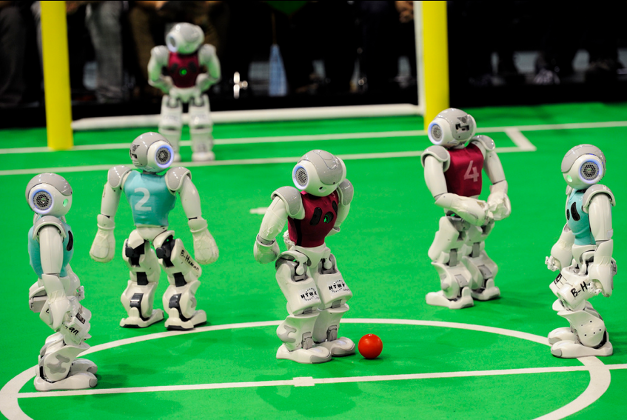
\includegraphics[width=\textwidth]{figures/intro_standard}
\caption[Robocup Soccer standard platform]{Two teams of Nao robots playing against each other in the 2014 edition of RoboCup Soccer standard platform league. \textit{[Photo courtesy of RoboCup]}}
\label{fig:intro_standard}
\end{subfigure}
\hfill
\begin{subfigure}[b]{0.45\textwidth}
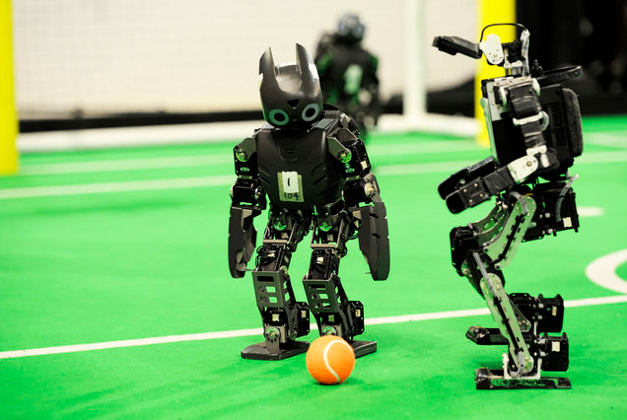
\includegraphics[width=\textwidth]{figures/intro_ks}
\caption[Robocup Soccer standard platform]{Two robots of opposing teams looking at the ball, in the 2013 edition of RoboCup Soccer kidsize league. \textit{[Photo courtesy of RoboCup]}}
\label{fig:intro_ks}
\end{subfigure}
\caption[Robocup standard and kidsize leagues]{Robocup standard and kidsize leagues}
\label{fig:intro_robocup}
\end{figure}

This contest is quite vast and, as of 2016, is divided into several categories (called domains in RoboCup jargon):
\begin{itemize}
\item RoboCup Rescue : as the name suggests, a domain where robots must perform various rescue operations in diverse scenarios.
\item RoboCup Industrial : a category with industrially oriented competitions, 
\item RoboCup@Home : centred around domestic robots, such as robotics helpers for the elderly or robotic butlers.
\item RoboCupJunior : more of an initiative that aims to foster robotics interest in children rather than a contest, it helps organize various robotics events for younger minds.
\item RoboCup Soccer : historically the first category, centred about humanoid robots playing football. The objective of this category is to have a team of robots beat the world champions by 2050. This is the category we will compete in.
\end{itemize}

RoboCup Soccer is further subdivided into 4 sub-categories called leagues :\begin{itemize}
\item Standard platform, where the teams all use the same robot, \emph{Nao}, as illustrated in \Cref{fig:intro_standard}.
\item Simulation, a league that does not feature physical robots but focuses on team strategies and artificial intelligence. The matches take place in 2D or 3D simulators.
\item Adultsize, for the taller robots.
\item Teensize, for middle sized robots.
\item Kidsize, for the smaller robots. \Cref{fig:intro_ks} shows robots from that league.
\end{itemize}

This year's team is preparing to participate to the Kidsize league and this master thesis, along with two others, is the by-product of that team's activity. Since this is our first time participating we have no experience regarding humanoids robots. To avoid spending countless hours building and testing different designs we need a tool able of simulating the physics of a robot model. 

\section{Goals of the project}
The goal of this thesis is to provide the team with a physics simulating tool with the following features :
\begin{itemize}
\item realistic simulation of the physics of rigid bodies. This means that the tool should handle inertia, collisions, friction and constraints between objects. Simulation of springs and dampers is an interesting bonus.
\item receive and process orders incoming at a relatively high frequency. The processing need not be in real-time.
\item the model of our robot should receive the same orders as the real robot would. That is, the simulator should provide the same interface to the control code as the real robot would. 
\item 3D visualization of the simulation.
\end{itemize}

That simulator will be used to :
\begin{enumerate}
\item Test different robot designs and choose the best one, in a more efficient way than it could be achieved by physically building the designs.
\item Speed up development and testing of the control code because multiple teams will be able to work in parallel. 
\end{enumerate}

\section{Structure of the report}
This report begins with an overview of the basic concepts behind physics simulation on computers in \cref{chap:principles}. We then move on to the chapter that motivates the choice of V-Rep as the main simulation tool for this project.

\Cref{chap:modelling} will be about the modelling of the build blocks of our humanoid robot. The verification and the tuning of the results of some basic simulations will be made in \cref{chap:physical_val}.

\Cref{chap:simulation} goes into the core of the subject with some simulations that influenced the design of the robot before being used to explore control strategies. The last chapter will conclude the work by summing up and laying out future prospects.